\documentclass[10pt]{article}
\usepackage[usenames]{color} %usato per il colore
\usepackage{amssymb} %maths
\usepackage{amsmath} %maths
\usepackage[utf8]{inputenc} %utile per scrivere direttamente in caratteri accentuati
\begin{document}
\[\section{External Interface Requirements}
	This section gives a description of the various inputs and relative outputs of the system. It also gives a description of the hardware, software and communication interfaces that are necessary to make the system work. It will also provide a generic visualization of the user interface in the various user platforms.

		\subsection{User Interfaces}
		Here we describe in particular how the application should look like either for mobile and web application. To make an easier explanation of the aspect of the various screen of the application we are going to use Mockup.
			\subsubsection{Login}
			On this page the users can log in with username and password or with Facebook (only if as registered user is a Customer). If the user is not already registered can access to the registration pages (for Customer or for Taxi Drivers). Also if the users forgot the password from this page can go to the forgot password page.
				
				\begin{figure}[H]
					\centering
					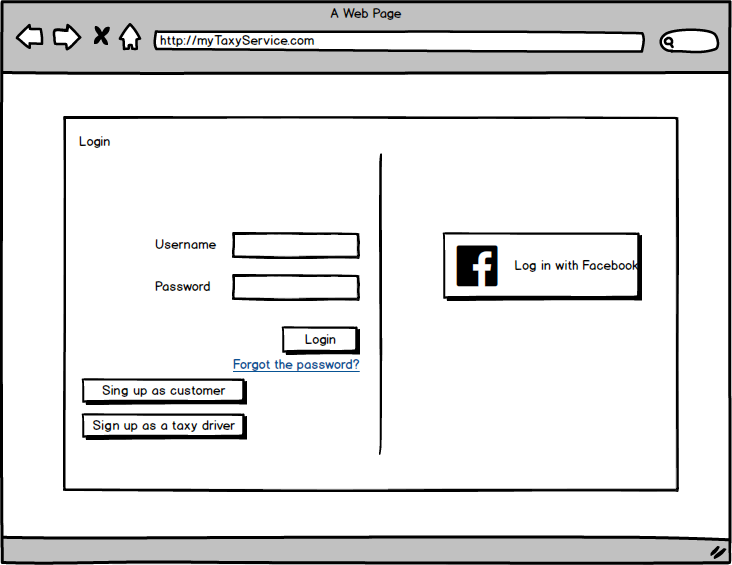
\includegraphics[scale=0.5]{IMG/UserInterfaces/CustomerLogin.png}
					\caption{Login Page, web version}\label{login_w}
				\end{figure}
				\begin{figure}[H]
					\centering
					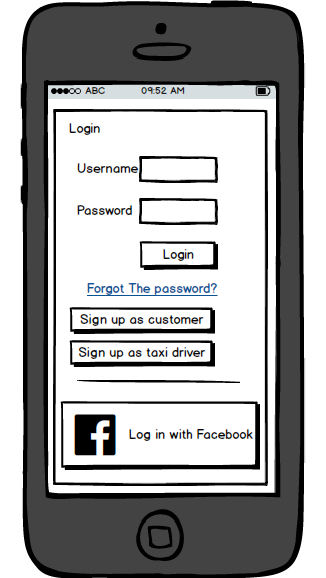
\includegraphics[scale=0.4]{IMG/UserInterfaces/CustomerLogin_m.png}
					\caption{Login Page, mobile version}\label{login_m}
				\end{figure}
			
			
			\subsubsection{Customer registration}
			On this page the users can register itself. This page must provide two way of registration, registration with the standard form ( e-mail, password and username) of with Facebook API.
			
				\begin{figure}[H]
					\centering
					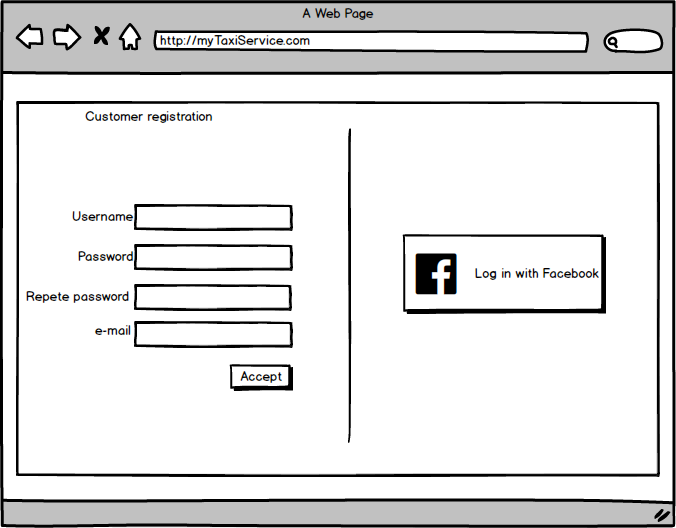
\includegraphics[scale=0.5]{IMG/UserInterfaces/CustomerRegistration.png}
					\caption{Customer registration Page, web version}\label{cregistration_w}
				\end{figure}
				\begin{figure}[H]
					\centering
					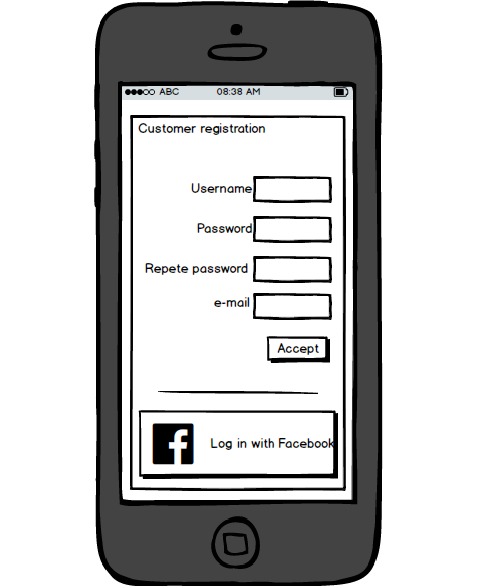
\includegraphics[scale=0.4]{IMG/UserInterfaces/CustomerRegistration_m.png}
					\caption{Customer registration Page, mobile version}\label{cregistration_m}
				\end{figure}
			
			\subsubsection{Taxi Drivers registration}
			On this page the users can register itself as a taxi driver. Taxi driver have a special form to been registered because of the additional information the user must provide (taxi license number). Just because the additional information the registration can be done just with the standard form.
				
				\begin{figure}[H]
					\centering
					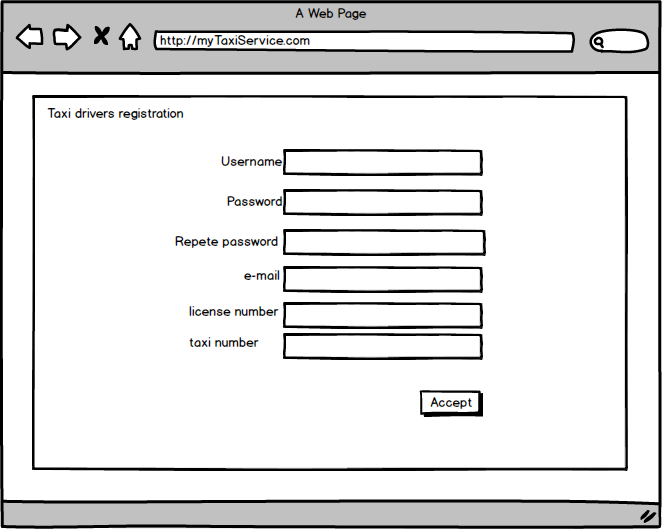
\includegraphics[scale=0.5]{IMG/UserInterfaces/TaxiDriverRegistration.png}
					\caption{Taxi Driver registration Page, web version}\label{tregistration_w}
				\end{figure}
				\begin{figure}[H]
					\centering
					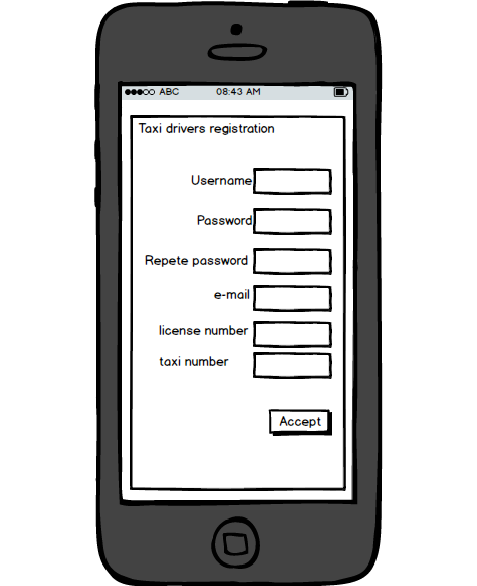
\includegraphics[scale=0.4]{IMG/UserInterfaces/TaxiDriverRegistration_m.png}
					\caption{Taxi Driver registration Page, mobile version}\label{tregistration_m}
				\end{figure}
			
			\subsubsection{Customer home page}
			On this page the Customer can see his position (information from his GPS) and perform all the main operation that he can perform. He can Request a taxi on the position showed, can go to the reservation page (in which can reserve a ride), can visit his personal page (in which can see all the information of his profile), can go to the information page (information about myTaxiService) or go to the 'my reservation page' (in which can manage all the previous reserved ride). 
			
				\begin{figure}[H]
					\centering
					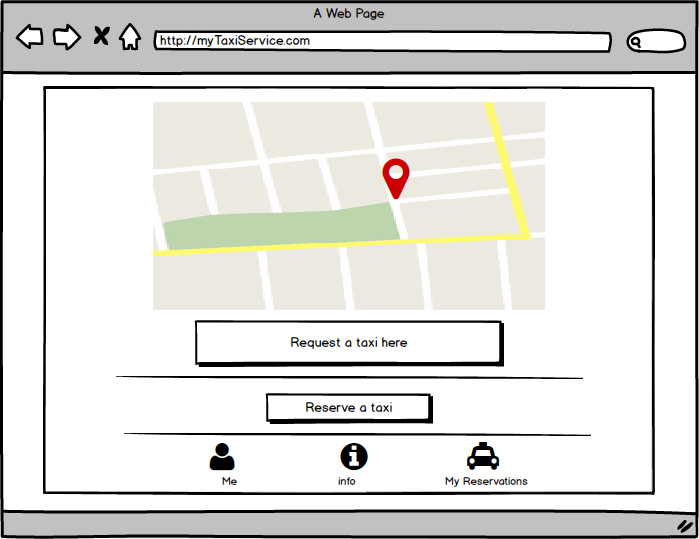
\includegraphics[scale=0.5]{IMG/UserInterfaces/mainCustomer.png}
					\caption{Customer home page, web version}\label{chome_w}
				\end{figure}
				\begin{figure}[H]
					\centering
					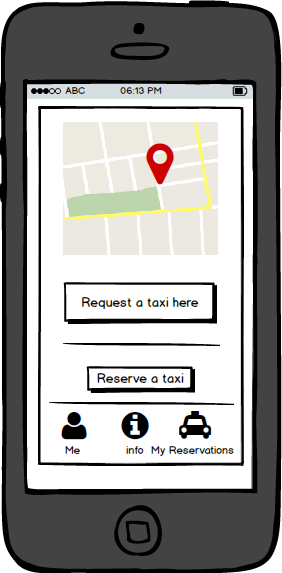
\includegraphics[scale=0.4]{IMG/UserInterfaces/mainCustomer_m.png}
					\caption{Customer home page, mobile version}\label{chome_m}
				\end{figure}
			
			\subsubsection{Reservation page}
			On this page the Customer can reserve a taxi ride. To do this he must insert a Origin position, a Destination position, a Data and a Time. The reservation must be at least two hours after the current Time, so the system must avoid to reserve a previous ride.
			
				\begin{figure}[H]
					\centering
					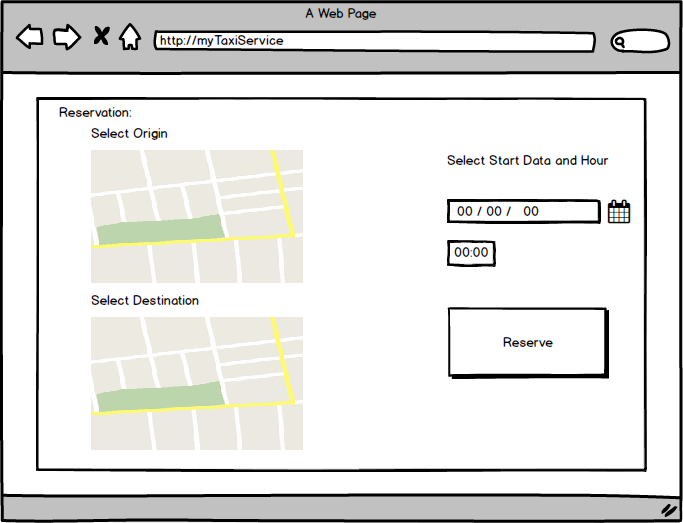
\includegraphics[scale=0.5]{IMG/UserInterfaces/reservationCustomer.png}
					\caption{Reservation page, web version}\label{reservation_w}
				\end{figure}
				\begin{figure}[H]
					\centering
					\includegraphics[scale=0.4]{IMG/UserInterfaces/reservationCustomer_m.png}
					\caption{Reservation page, mobile version}\label{reservation_m}
				\end{figure}
			
			\subsubsection{My reservation Page}
			On this page Customer can see all the reservation he have already done and adding some new. For each previous reservation can see all the information and, if the Date is before the next two hours, can delete it.			
			
				\begin{figure}[H]
					\centering
					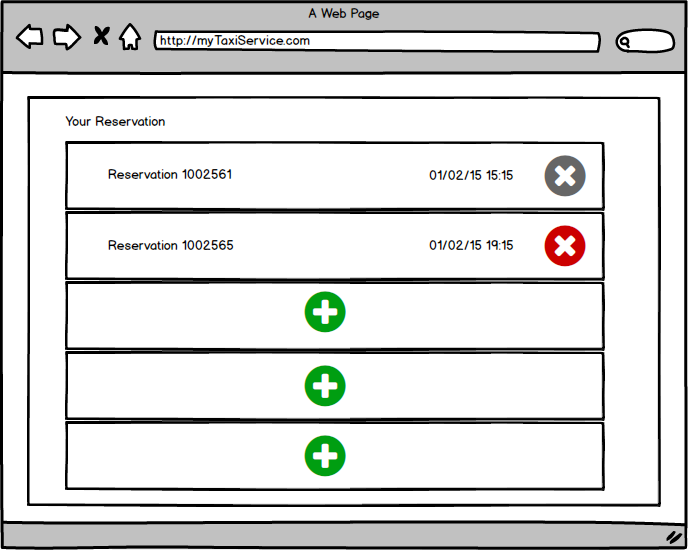
\includegraphics[scale=0.5]{IMG/UserInterfaces/myReservation.png}
					\caption{My reservation, web version}\label{myreservation_w}
				\end{figure}
				\begin{figure}[H]
					\centering
					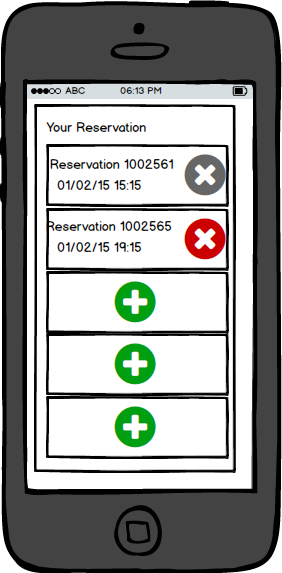
\includegraphics[scale=0.4]{IMG/UserInterfaces/myReservation_m.png}
					\caption{My reservation, mobile version}\label{myreservation_m}
				\end{figure}
			
			
			\subsubsection{Customer notification pop-up}
			This pop-up is showed to the requesting Customer when his request has been handled. On this pop-up the system show also the number of the incoming taxi and an approssimative waiting time.
			
				\begin{figure}[H]
					\centering
					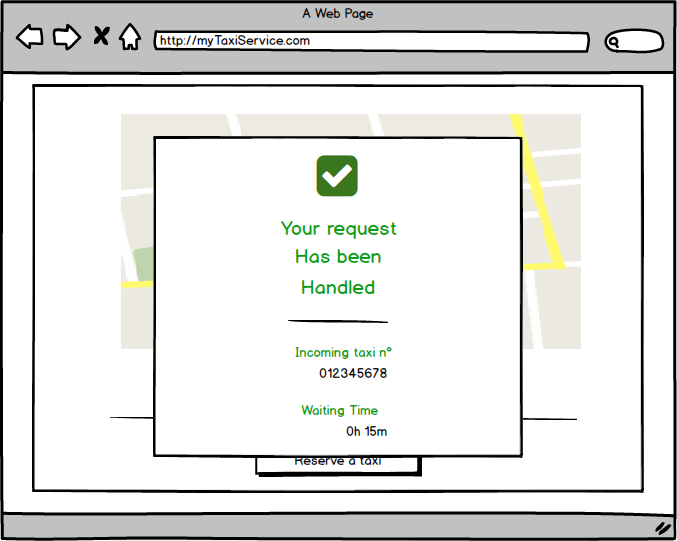
\includegraphics[scale=0.5]{IMG/UserInterfaces/customerNotification.png}
					\caption{Customer nofication, web version}\label{requestHandlded_w}
				\end{figure}
				\begin{figure}[H]
					\centering
					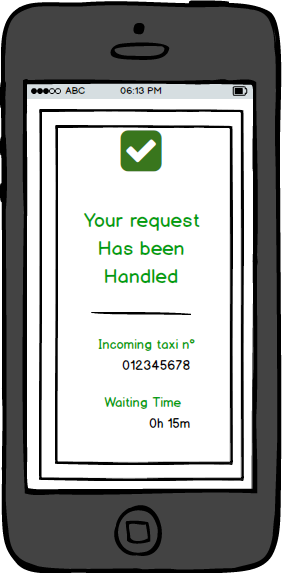
\includegraphics[scale=0.4]{IMG/UserInterfaces/customerNotification_m.png}
					\caption{Customer notification, mobile version}\label{requestHandled_m}
				\end{figure}
			
			\subsubsection{User page}
			This page show all the information about your user and show how many time you've been notified as bad user.
			
				\begin{figure}[H]
					\centering
					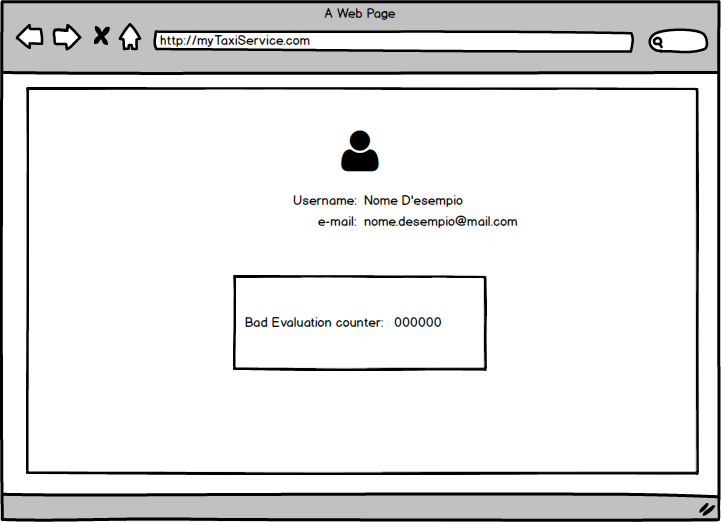
\includegraphics[scale=0.5]{IMG/UserInterfaces/userPage.png}
					\caption{User Page, web version}\label{cpersonalPage_w}
				\end{figure}
				\begin{figure}[H]
					\centering
					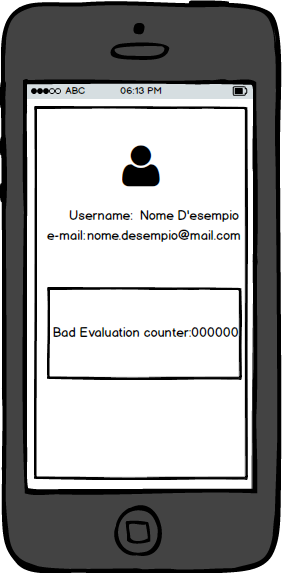
\includegraphics[scale=0.4]{IMG/UserInterfaces/userPage_m.png}
					\caption{User Page, mobile version}\label{cpersonalPage_m}
				\end{figure}

			
			\subsubsection{Taxi Driver home page}
			On this page the Taxi driver can see his position (information from his GPS) and inform the system about his availability.
			
				\begin{figure}[H]
					\centering
					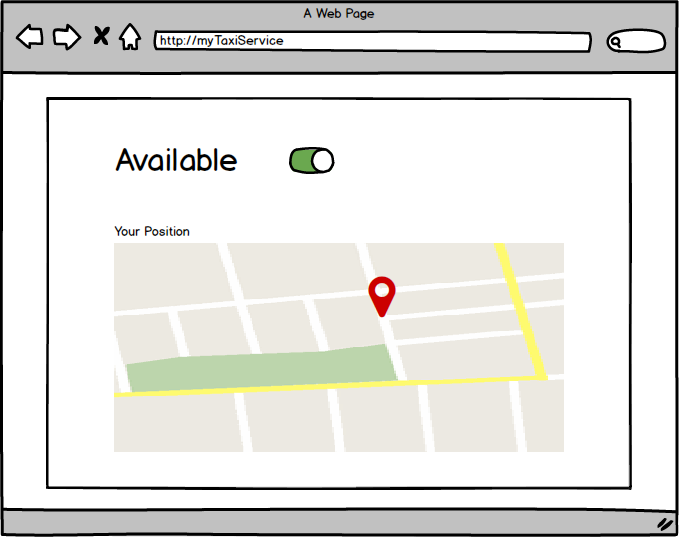
\includegraphics[scale=0.5]{IMG/UserInterfaces/mainTaxiDriver.png}
					\caption{Taxi driver home page, web version}\label{thomePage_w}
				\end{figure}
				\begin{figure}[H]
					\centering
					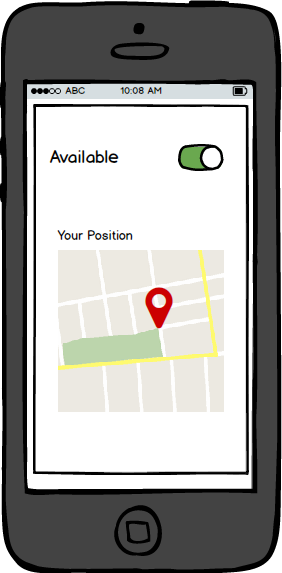
\includegraphics[scale=0.4]{IMG/UserInterfaces/mainTaxiDriver_m.png}
					\caption{Taxi driver home page, mobile version}\label{thomePage_m}
				\end{figure}
			
			
			
			\subsubsection{Taxi Driver notification}
			On this pop-up the taxi driver will notified of a request that he can handle. On this pop-up is showed also two button, with which the taxi driver can accept or decline the request.
			
				\begin{figure}[H]
					\centering
					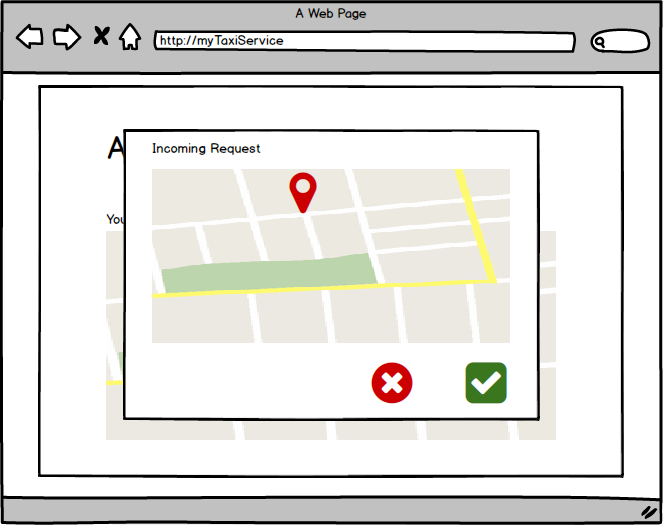
\includegraphics[scale=0.5]{IMG/UserInterfaces/notificationTaxiDriver.png}
					\caption{Taxi driver notification pop-up, web version}\label{requestNotification_w}
				\end{figure}
				\begin{figure}[H]
					\centering
					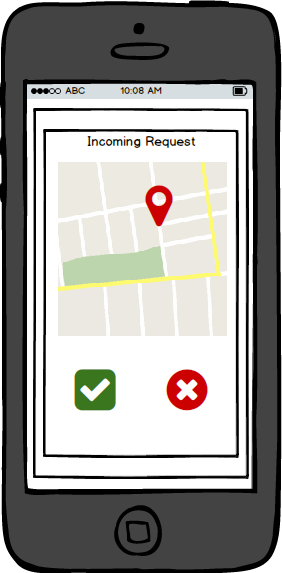
\includegraphics[scale=0.4]{IMG/UserInterfaces/notificationTaxiDriver_m.png}
					\caption{Taxi driver notification pop-up, mobile version}\label{requestNotification_m}
				\end{figure}
				
			
			\subsubsection{Registered user end ride page}
			When a taxi driver accept a ride this page is showed up to each registered user involved in this ride. On this page the taxi driver can check the name of the customer and the Origin position of his journey. When the ride is ended each of the registered user can give a bad evaluation to the other or simply end the ride and return to the main page.
				
				\begin{figure}[H]
					\centering
					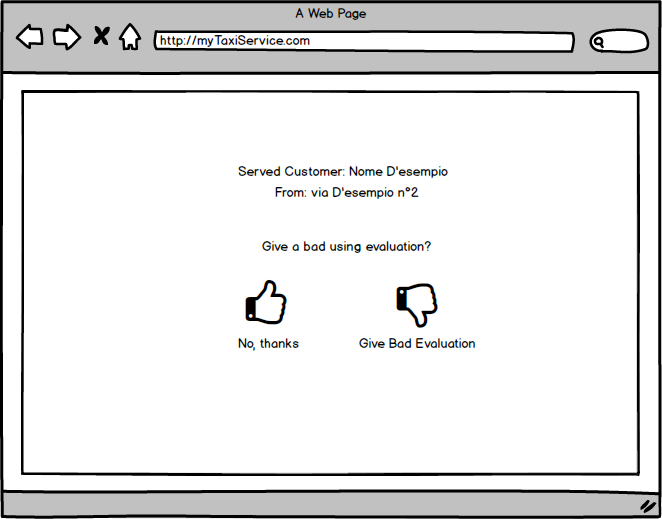
\includegraphics[scale=0.5]{IMG/UserInterfaces/onRidePage.png}
					\caption{On Ride Page, web version}\label{tendRidePage_w}
				\end{figure}
				\begin{figure}[H]
					\centering
					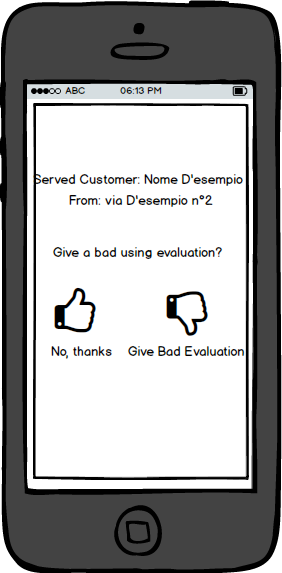
\includegraphics[scale=0.4]{IMG/UserInterfaces/onRidePage_m.png}
					\caption{On Ride page, mobile version}\label{tendRidePage_m}
				\end{figure}
				

		\subsection{Hardware Interfaces}
		Since mobile and web applications don't have any dedicated hardware we have not designed any hardware interfaces for our system.
		The interaction with the central database is performed by connections handled by the already installed operating system on the mobile devices or the users computers.

		\subsection{Software Interfaces}
			\begin{itemize}
				\item The mobile application communicates with the GPS application in order to get geographical informations about the user.
				
				\item The web application communicates with the browser in order to get geographical informations about the user.
				
				\item Mobile and web applications communicates with the database through HTTP requests to the server.
			\end{itemize}

		\subsection{Interfaces to Others Application}
			\begin{itemize}
				\item myTaxiService web application require that at least one of these browsers is installed on the user Personal Computer:
			
					\begin{center}
						\begin{table}[h!]
							
							\begin{center}
								\caption{Browsers}
								\label{tab:browsersTable}

								\begin{tabular}{cccc}
									\toprule
									\textbf{Name} & \textbf{Version} & \textbf{Company} & \textbf{Source}\\
									\midrule
									Safari & 9.0.1 & Apple Inc. & \href{http://www.apple.com/safari/}{Get Safari}\\
									\midrule
									Firefox & 41.0 & Mozilla & \href{https://www.mozilla.org/en-US/firefox/new/}{Get Firefox}\\
									\midrule
									Chrome & 46.0.2490 & Google & \href{https://www.google.com/chrome/browser/desktop/}{Get Chrome}\\
									\midrule
									Microsofr Edge & 20.10240.16384.0 & Microsoft & \href{https://www.microsoft.com/en-us/download/details.aspx?id=48126}{Get Edge}\\
									\bottomrule
								\end{tabular}
							\end{center}
							
						\end{table}
					\end{center}

				\item myTaxiService mobile application require that at least one of these operating systems is installed on the user Smartphone:

					\begin{center}
						\begin{table}[h!]
							
							\begin{center}
								\caption{Mobile Operative Systems}
								\label{tab:mobileOSTable}

								\begin{tabular}{cccc}
									\toprule
									\textbf{Name} & \textbf{Version} & \textbf{Company} & \textbf{Source}\\
									\midrule
									Android & KitKat 4.4W.2 or later & Google & \href{https://www.android.com}{Android Info}\\
									\midrule
									iOS & 9.1 or later & Apple Inc. & \href{http://www.apple.com/ios/}{iOS Info}\\
									\midrule
									Windows 10 & 10.0.10572.0 or later & Microsoft & \href{http://www.microsoft.com/it-it/mobile/windows10/?dcmpid=omc-org-globalsite.globalredirect}{Windows 10 Info}\\
									\bottomrule
								\end{tabular}
							\end{center}
							
						\end{table}
					\end{center}

				\item To give an additional LogIn method, we use also the "LogIn with Facebook" API relased by Facebook. Facebook Login for Apps is a fast and convenient way for people to create accounts and log into our system across multiple platforms. It is well described at \href{https://developers.facebook.com/docs/facebook-login}{Facebook Login API Page.}
			\end{itemize}


		\subsection{Communication Interfaces}
		The communication between system pieces is not specified because it is handled by the underlying operating systems for both the mobile application and the web portal.

		In particular, the web and mobile applictaions will communicate with the server through HTTP/HTTPS requests. 

			\begin{itemize}
				\item HTTP communicate through the port number 80 and is handled by the operating system. 
				\item HTTPS communicate through the port number 443 and is handled by the operating system.
			\end{itemize}\]
\end{document}